% vim:set et sw=2 ts=4 tw=72:
\chapter{Introduction}

Visualizations of the directed acyclic graph of an active software
system repository are difficult to understand. These visualizations are
used to provide information about the topology of the repository, which
gives insight on how commits are being integrated. Maintainers must use
this information to understand the changes that are being made to the
current version of the software, so that the fixes can be applied to
older versions as well. This requires them to understand how the commit
with the necessary changes are integrated, and identifying other commits
that are necessary for this integration to take place. In large software
repositories, this task is not trivial. This \paper{} presents the
design of a new model constructed from the underlying graph of the
repository.

The work in this \paper{} focuses on the Linux repository, which uses
git for managing changes in the code and helping coordinate
contributors. Linux is highly active, with more than 8,000 commits added
per release. Linux is used in many software applications, including
mobile phones, smart appliances, and even spacecraft. Maintainers must
be able to port the patches to the current version of the kernel back
into the version of the kernel that they are maintaining. This requires
them to determine which commits are relevant to them, and how these
commits are integrated. This work was originally motivated by the
request of an external industrial entity, requesting a means of
visualizing how commits are integrated. \evan{keep this or leave it out?}

Git is a distributed version control system that uses the directed
acyclic graph (DAG) model to store modifications to code in nodes, and
help with branching and merging related changes. Git was designed by
Linus Torvalds in 2005 specifically for the needs of the Linux kernel
repository after the Linux project switched from Bitkeeper. Since git
was designed for the Linux project, the repository makes use of nearly
every feature in git. The DAG model allows git to have impressive
flexibility compared to many other version control systems, but suffers
from poor visualizations. In large projects, the visualizations of the
DAG do not provide an adequate summarization of how a commit is
integrated into the master branch of a repository.

While there has been extensive research on visualizing software
repositories, previous work does not focus on the topology of the
repository, and in extension, how a commit is integrated. The literature
on repository visualization and summarization can be broken down into
three main subcategories; communication\cite{Cubranic2005,Begel2010},
aspect-oriented visualization\cite{Ambros2005,Burch2005,Ambros2009}, and
organic visualizations\cite{ogawa09,Caudwell2010}. A fourth category can
be added to include non-academic tools, like GitKraken and SourceTree,
built as clients to work with git repositories and visualize the DAG
model directly. The goals of these tools is not to extract new
information from the repository, but to act as a user-friendly client on
top of git.

This \paper{} introduces a new model designed to help clearly visualize
the path that a commit takes to being integrated into the master branch.
To test the viability of the model, I build and evaluate a tool called
\tool{}, which is designed to leverage the capabilities of the \mt{} to
provide improved summarizations and visualizations of the merges in
Linux. When constructing and evaluating the model and tool, three
questions arose; first, we want to ensure that the visualizations of the
directed acyclic graph (DAG) do not already provide meaningful
summarization of how a commit is integrated (RQ\ref{rq:RQ1}). Next, we
want to compare the visualization of the DAG against the visualization
of the \mt{} to determine which is capable of providing a better
understanding of how a commit is integrated (RQ\ref{rq:RQ2}). Finally,
the new model should make it possible to more easily extract additional
aggregate information about what is being integrated, and who is making
the contributions (RQ\ref{rq:RQ3}).

%% TODO: Move to methodology section
\begin{textbox}
  \textbf{RQ\rqs{rq:RQ1}:} Do visualizations of the DAG provide
  users with a meaningful visualization of how commits are integrated?
\end{textbox}

\evan{Not sure about the first research question. Its essentially
  motivation. ``What are weaknesses in the DAG visualizations'' might be
  better. That was found in the Conceptual understanding part. ``Does
  the DAG provide users with meaningful visualization of small merges''}

\begin{textbox}
  \textbf{RQ\rqs{rq:RQ2}:} How does the visualization of the \mt{}
  compare with the visualization of the DAG to determine how commits are
  integrated?
\end{textbox}

\begin{textbox}
  \textbf{RQ\rqs{rq:RQ3}:} What other information can be drawn from the
  \mt{} model that cannot easily be drawn from the DAG.
\end{textbox}

%% TODO: More is described in the background section of the paper

\section{Related Work}\label{sec:related_work}

The \define{Version Control System}{VCS} tracks the development of a
software project, recording each change as it happens. In many cases,
the VCS contains the entire story of the software, with rich information
about the authors, files, and changes being made. This makes the VCS
vital in providing information about how a software project is being
developed, how the software is structured, and extending Conway's law,
can reflects the communication structure within an organization. In
order to use the information stored in the VCS, users must be able to
gain a clean understanding and summarization of the changes being made
and how they interact with the rest of the source code. Various
visualizations of have been written to tackle various aspects of this
challenge, but we are aware of no git repository visualization tool that
was designed with the explicit goal of showing how commits are
integrated into the master branch of the repository. There has, however,
been a lot of work in providing visualizations of various aspects of a
repository.

Many tools focus on addressing the issue in communication between
developers in inter-team collaborative work. Hipikat\cite{Cubranic2005}
investigates communication between developers, focusing on assisting
with the integration of new developers into a project though
communication, providing the new developer with searchable artifacts of
the changes being made, and where to find them. Codebook\cite{Begel2010}
also focuses on communication, but where Hipikat focuses on assisting
new developers find artifacts, Codebook assists developers with finding
who was responsible for creating the artifact. Codebook uses a
data-mining technique to determine the developer of a piece of code, the
program manager who wrote the specification for the code, and the
program managers and developers on the team who were working together.
Neither tool is designed with the goal of providing information on the
topological structure of a source code repository, nor are these tools
designed for visualization purposes.

Most visualization systems provide information about a certain aspect of
the contents in the repository. Fractal Figures\cite{Ambros2005} uses a
square to represent a component of a project. Then subdividing the
square based on the proportion of an author's contributions to that
component. EPOSee\cite{Burch2005} and Evolution Radar\cite{Ambros2009}
perform further analysis to determine which files are created together,
and see what changes are made over a sequence of commits. The goals of
these two projects differ slightly, but both use evolution over time to
extract information about how different parts of a software system are
related.

Codebook, Hipikat, Fractal Figures, EPOSee, and Evolution Radar all
extract data from CVS repositories. Our goal is to provide information
about git repositories. Fewer tools are available for generating
visualizations and summaries of git repositories, potentially due to the
DAG model used as the internal structure of git repositories.

Heller et al.\cite{Heller2011} apply geo-spatial information to the
commits in git repositories to see organic patterns that arise in
collaboration between contributors to a repository.
Gource\cite{Caudwell2010} is a tool for providing an interactive
timelapse of the changes being made to various files stored in the
repository. Gource uses a graph metaphor for representing the file
structure in the repository. Files are the nodes in the graph, and the
clustering of the file represents directories. The edges are the links
between directories. User avatars move around the graph emitting
different color light depending on the change being made to the file.
Green indicates the creation of a new file, yellow indicates a
modification, and red indicates the deletion of the file (shown in
Figure~\ref{fig:gource_view}). Codeswarm\cite{ogawa09} is similar to
Gource, using an organic timelapse approach to visualizing the events in
the repository. Unlike Gource, which focuses on files, Codeswarm focuses
on developers and the number of commits each developer is making.

\begin{figure}[htpb]
  \centering
  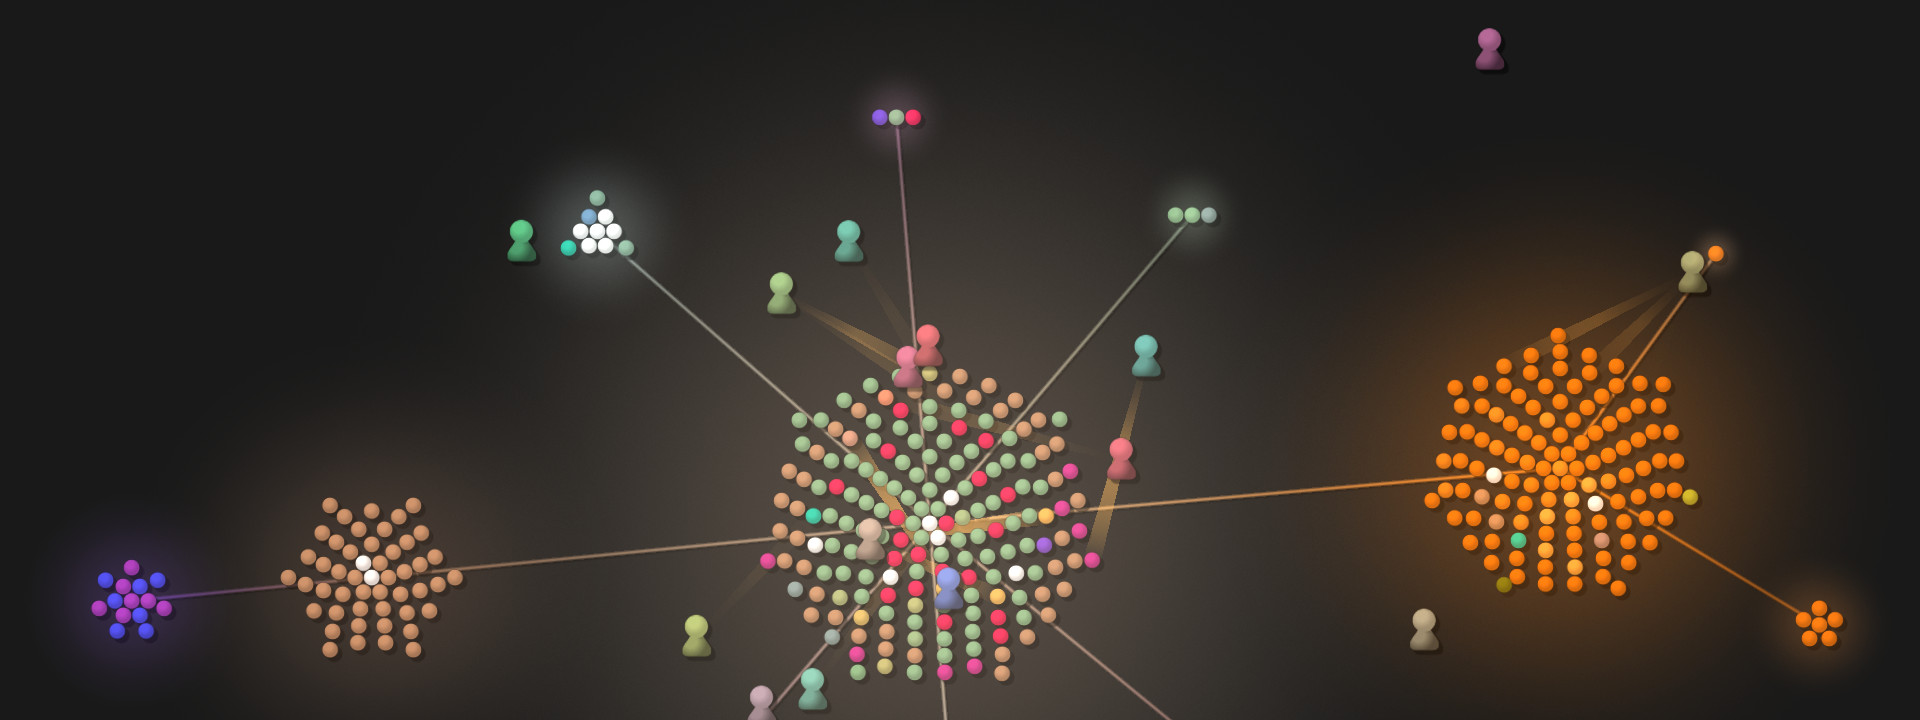
\includegraphics[width=0.8\linewidth]{./Figures/introduction/gource-linux.jpg}
  \caption{View of Gource file graph with users operating on a
    repository}
  \label{fig:gource_view}
\end{figure}

There are many non-academic programs that are designed as an interface
to git. While not all of these programs provide visualizations, those
that do use a visual metaphor of the DAG to show topological information
about the repository. Some of the interfaces are shown in
Figure~\ref{fig:non_academic_work}. While they ultimately show the same
information, the topology of the repository, the organization of that
information is different. GitKraken is a popular commercially written
git interface that aims to be efficient, elegant, and reliable,
according to the GitKraken website. On visual inspection, it appears to
be all of these things. GitLab and GitHub are both online repository
hosts, with visualization and summarization provided as well. While the
GitLab visualization does not appear to provide any additional
information, the GitHub visualization does take advantage of it's
internal knowledge of forks. Through this visualization, GitHub displays
the branch history of the repository network, including the branches of
the main repository and forks from that. Giteye and most of the other
visualizations are relatively conventional, simply cleaning up the
interface of Gitk, the visualizer that is shipped with git. With the
exception of Gitk, no GUI visualizers are able to produce a
visualization for the Linux repository, due to its size. The GitHub
visualizer displays an error message, stating that there are too may
forks to display. The GitKraken interface will freeze and eventually
crash while trying to load the repository, while Giteye and the other
visualizers will consume all of the system memory before they are able
to produce a visualization. The Gitk interface is the least polished,
but is able to produce a visualization of the repository.

\begin{figure}[htpb]
  \centering
  \begin{tabular}{cc}
    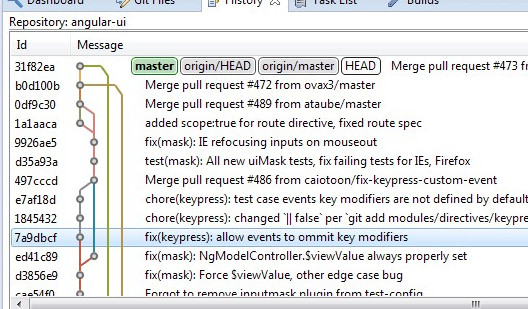
\includegraphics[height=3.5cm]{Figures/introduction/giteye_graph.jpg}
    &
    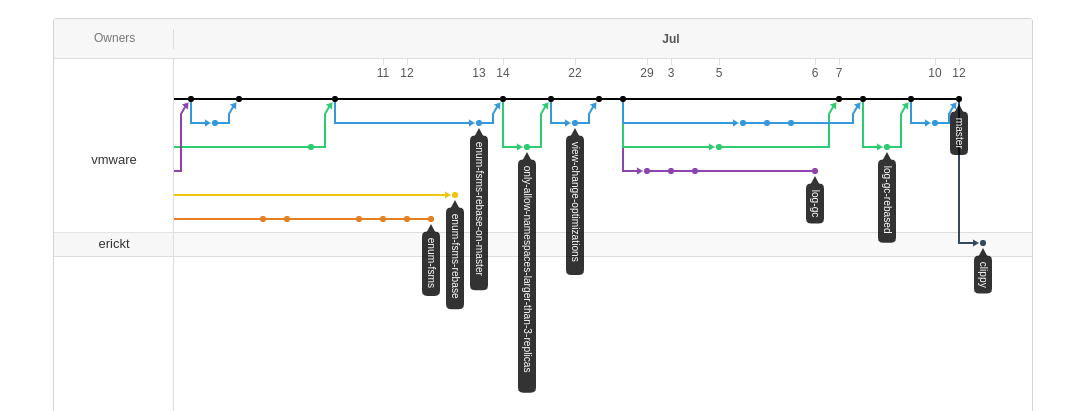
\includegraphics[height=3.5cm]{Figures/introduction/github_dag.png}
    \\

    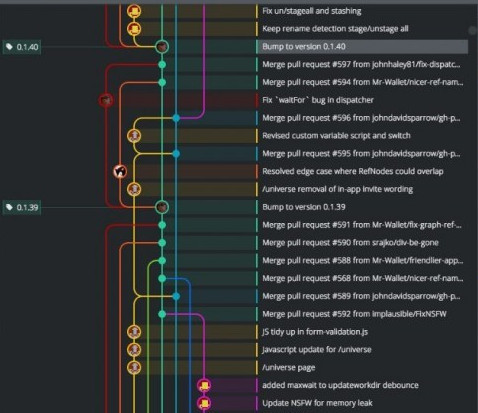
\includegraphics[height=3.5cm]{Figures/introduction/gitkraken_graph.jpg}
    &
    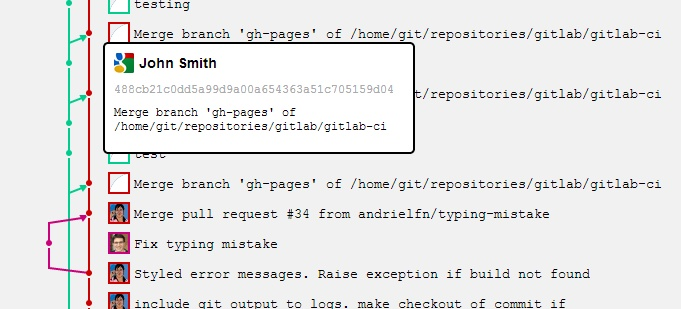
\includegraphics[height=3.5cm]{Figures/introduction/gitlab_graph.jpg}
  \end{tabular}

  \caption{Various non-academic git interfaces. In clockwise order from the
    top-left; Giteye, Github, Gitlab, and GitKraken.}
  \label{fig:non_academic_work}
\end{figure}
